\subsection{Возможности языка}
Язык "<jetbrains.mps.baseLanguage.stateMachine"> (далее "<stateMachine">) представляет собой автоматное расширение языка "<baseLanguage">. Основная цель, которая приследовалась при разработке языка "<stateMachine">, --- создать средство, позволяющее описывать поведение классов в виде автоматов, не накладывая на сами классы никаких дополнительных ограничений. Более того, автоматное описание поведения класса должно быть инкапсулировано. То есть код, использующий класс не должен "<знать"> о том, каким образом задано поведение класса. Этот подход отличается от предложенного в работе \cite{myUMLSwitchEclipse} тем, что позволяет использовать автоматы не только в программах написанных в соответствии со SWITCH-технологией, но и в традиционных объектно-ориентированных программах.

В качестве примера использования языка "<stateMachine"> взята система управления лифтом \cite{knuth}. Используемая реализация системы является упрощенным решением задачи управления лифтом, описанном в работе \cite{naumov}. Логика управления всеми подсистемами лифта реализована в одном автомате.

Каждый автомат в языке "<stateMachine"> связан с некторым классом и описывает его поведение. Для удобства редактирования автомат описывается в отдельном корневом узле \pic{\ref{fig:ElevatorStateMachine}}.

\begin{figure}
 \centering
 \fbox{
  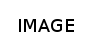
\includegraphics[width=0.9\textwidth]{placeholder.png}
 }
 \caption{Фрагмент автомата управляющего лифтом}
 \label{fig:ElevatorStateMachine}
\end{figure}

Для того чтобы задать поведение класса с помощью автомата в языке "<stateMachine"> необходимо в этом классе определить события, на которые будет реагировать автомат. Особенностью языка "<stateMachine"> является то, что события в нем --- это методы специального вида. В языке "<Java"> декларации методов различаются по способу реализации:
\begin{itemize}
 \item обычные методы, реализация которых следует сразу за объявлением метода;
 \item нативные методы, реализованные на платформо-зависимых языках программирования;
 \item абстрактные методы, вообще не имеющие реализации.
\end{itemize}
Событие в языке "<stateMachine"> --- это метод, реализация которого находится в автомате и зависит от текущего состояния автомата. Например, в классе "<Elevator"> объявлены следующие события \pic{\ref{fig:ElevatorEvents}}
\begin{description}
 \item[doorsOpened, doorsClosed] --- события, которые посылает объект управления "<DoorsEngine">, когда двери оказываются в максимально открытом и полностью закрытом положении соответственно;
 \item[floorReached] --- событие, которое посылает объект управления "<ElevatorEngine">, когда лифт достигает очередного этажа;
 \item[call] --- событие, которое получает автомат, когда пассажир нажимает кнопку вызова лифта на этаже, или в кабине лифта;
 \item[openDoors] --- событие, которое получает автомат, когда пассажир нажимает кнопку экстренного открывания дверей в кабине лифта;
 \item[loadingTimeout] --- событие, которое посылает объект управлени "<LoadingTimer">, когда истекает время ожидания погрузки пассажиров.
\end{description}
\begin{figure}
 \centering
 \fbox{
  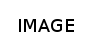
\includegraphics[width=0.9\textwidth]{placeholder.png}
 }
 \caption{События автомата управляющего лифтом}
 \label{fig:ElevatorEvents}
\end{figure}
Так как события являются обычными методами, их можно использовать в качестве реализации абстрактных методов. Это позволяет уменьшить количество зависимостей в программе. Например, объект управления "<ElevatorEngine"> не имеет непосредственных ссылок на класс "<Elevator">. Вместо этого в программе объявлен интерфейс "<ElevatorEngineListener">, и объект управления "<ElevatorEngine"> извещает о событиях экземпляры этого интерфейса. Класс "<Elevator"> реализует интерфейс "<ElevatorEngineListener"> и поэтому может обрабатывать события объекта управления "<ElevatorEngine">. Таким образом удается классически реализовать паттерн проектирования "<Обозреватель"> \cite{gof}.

Реакция автомата на событие зависит от состояния, в котором автомат находится. Состояния автомата бывают двух типов: обычные и конечные. Конечные состояния отличаются тем, что не могут иметь исходящих переходов. То есть, когда автомат оказывается в конечном состоянии он перестает обрабатывать события.

Первое состояние, объявленное в автомате, считается начальным. При создании экземпляра класса, для которого определен автомат, после выполнения конструктора осуществляется переход в начальное состояние.

Обычные состояния могут быть вложены друг в друга. При этом, если состояние содержит

События, как и другие методы, могут иметь формальные параметры. Значения этих параметров доступны в условиях и действиях на переходах.



Каждый автомат в языке "<stateMachine"> связан с некоторым классом, имеет доступ к полям и может вызывать методы этого класса. Поэтому в языке "<stateMachine"> нет необходимости в специальных конструкциях для взаимодействия между автоматами, так как вместо вложения одного автомата в другой можно использовать агрегацию одного класса с автоматом, другим классом с автоматом, а посылка события из одного автомата в другой ни что иное как вызов метода.